\documentclass[11pt,a4paper]{article}

\usepackage[margin=2.5cm]{geometry}
\usepackage{amsmath,amssymb,amsthm}
\usepackage{graphicx}
\usepackage{booktabs}
\usepackage{enumitem}
\usepackage{microtype}
\usepackage[hidelinks]{hyperref}
\usepackage{xcolor}
\hypersetup{pdftitle={A Census of Multi-Colour Langton's Ants up to Twelve Colours, with an Exact Escape Formula and a Highway Proof for the Family L^(K-1)R},pdfauthor={Vishnu Vaidyanathan}}

\newtheorem{theorem}{Theorem}
\newtheorem{lemma}[theorem]{Lemma}
\newtheorem{corollary}[theorem]{Corollary}
\theoremstyle{definition}
\newtheorem{definition}[theorem]{Definition}
\newtheorem{observation}[theorem]{Observation}
\theoremstyle{remark}
\newtheorem{remark}[theorem]{Remark}

\newcommand{\Lw}{\mathtt{L}}
\newcommand{\Rw}{\mathtt{R}}
\newcommand{\w}[1]{\texttt{#1}}
\newcommand{\Z}{\mathbb{Z}}

\title{A Census of Multi-Colour Langton's Ants up to Twelve Colours,\\
with an Exact Escape Formula and a Highway Proof\\ for the Family $\Lw^{K-1}\Rw$}
\author{Vishnu Vaidyanathan\\[2pt]
\small ORCID: \href{https://orcid.org/0009-0001-6244-5262}{0009-0001-6244-5262}}
\date{November 2026}

\begin{document}
\maketitle

\begin{abstract}
A multi-colour Langton's ant is given by a rule string of $K$ letters $\Lw$ and $\Rw$.
We run every rule string with $K = 2$ to $12$ colours for one million steps and sort the
$4{,}015$ distinct machines that remain, after removing mirror images and repeated strings, by the
shape they grow: $2{,}723$ chaotic, $790$ square, $416$ highway, $83$ symmetric and $3$ triangle.
Every symmetric machine has a rule whose runs of equal letters, read in a circle, all have even length.
We show that $164$ of the highway machines never read the last letters of their rule and walk the same
path as another machine, leaving $252$ different highway paths, and that highways starting with
$\Rw$ in second place do not occur for fewer than seven colours.
Our main result concerns the family $A_K = \Lw^{K-1}\Rw$. We prove that, for every $K \ge 3$,
$A_K$ makes exactly $7{,}488$ right turns, at the same squares and in the same directions for every $K$,
before it first leaves the square box of side $2{,}998$ around its start (the edge, Section~\ref{sec:defs}),
which happens at step
$26{,}969 + 11{,}980\,(K-3)$, and that it then builds a diagonal highway forever, advancing two
squares diagonally every $16K - 12$ steps.
The proof is a single computer run in which $K$ is kept as a symbol: every square's colour is stored
as an affine expression $a + bK$, and every spin of the ant round a $2 \times 2$ loop is jumped over in
one step. All code and data are public.
\end{abstract}

\noindent\textbf{Keywords:} Langton's ant, turmites, cellular automata, highway, symbolic simulation,
computer-assisted proof.\\
\textbf{MSC 2020:} 37B15, 68Q80.

\section{Introduction}

Langton's ant~\cite{langton} is a single head moving on an infinite square grid of white squares.
On a white square it turns right, on a black square it turns left; it then flips the colour of the square
and steps forward. Starting from an all-white grid, it wanders chaotically for about $10{,}000$ steps
and then builds a ``highway'': a pattern that repeats every $104$ steps and moves diagonally away
forever. That the ant always escapes to infinity is a theorem~\cite{bunimovich}; that it always ends on a
highway, from any finite starting pattern, is still open. The ant is also capable of universal
computation~\cite{gajardo}, so questions about its long-run behaviour are hard in general.

Turk and Propp generalised the ant to $K$ colours~\cite{dewdney,gale}. A rule string
$w = w_0 w_1 \cdots w_{K-1}$ of letters $\Lw$ and $\Rw$ says which way to turn on each colour; the
square's colour then advances by one, modulo $K$. The classic ant is $\Rw\Lw$. Gale, Propp, Sutherland
and Troubetzkoy~\cite{gale} studied these ants and showed that rules built from repeated pairs of
letters give symmetric patterns. Many individual rules are known for their pictures: $\Lw\Lw\Rw\Rw$
grows a symmetric shape, $\Lw\Rw\Rw\Rw\Rw\Rw\Lw\Lw\Rw$ fills a square, and
$\Rw\Rw\Lw\Lw\Lw\Rw\Lw\Lw\Lw\Rw\Rw\Rw$ grows a triangle.

We were not able to find a complete table of how often each kind of shape occurs for each number of
colours. This paper gives one for $K \le 12$ (Section~\ref{sec:census}), reports patterns in the rule
strings that predict the shape (Section~\ref{sec:obs}), and then proves an exact result for the infinite
family $A_K = \Lw^{K-1}\Rw$ (Sections~\ref{sec:family} and~\ref{sec:proof}). The proof method,
running the ant once with $K$ as a symbol, may apply to other families.
Throughout, the census results are \emph{experimental}: they describe each machine after a fixed
number of steps and depend on our classification tests. Theorem~\ref{thm:main} and the lemmas of
Sections~\ref{sec:copies} and~\ref{sec:proof} are \emph{proved}.

\section{Definitions}\label{sec:defs}

\begin{definition}[Ant]
A \emph{rule} is a string $w = w_0 \cdots w_{K-1} \in \{\Lw,\Rw\}^K$, $K \ge 2$. A \emph{state}
is a position $p \in \Z^2$, a direction $d \in \{0,1,2,3\}$ (up, right, down, left) and a colouring
$\sigma : \Z^2 \to \{0, \dots, K-1\}$ that is $0$ on all but finitely many squares. One \emph{step}
reads $c = \sigma(p)$, turns right ($d \leftarrow d+1 \bmod 4$) if $w_c = \Rw$ and left
($d \leftarrow d - 1 \bmod 4$) if $w_c = \Lw$, sets $\sigma(p) \leftarrow c+1 \bmod K$, and moves
$p$ one square in direction $d$. We use screen coordinates: up is $(0,-1)$, right is $(1,0)$.
The ant starts at $p = (0,0)$, facing up, with $\sigma \equiv 0$.
\end{definition}

Since every visit adds one to the colour, $\sigma(p)$ is the number of visits to $p$ so far, modulo $K$.
On its $n$-th visit to a square the ant reads letter $w_{(n-1) \bmod K}$.

\begin{definition}[Reaching the edge]
Let $B = \{(x,y) : -1499 \le x \le 1498,\ -1499 \le y \le 1498\}$.
The ant \emph{reaches the edge at step $t$} if the move made in step $t$ (steps counted from $0$) is
the first to take it outside $B$. This is the same as running on a $3000 \times 3000$ grid started
at its centre and stopping one square from its border; all step counts in this paper use it.
\end{definition}

\paragraph{Machines that are the same.} Two rules can give the same ant:
\begin{itemize}[nosep]
\item \emph{Mirror twins.} Swapping every $\Lw$ and $\Rw$ gives the mirror image of the same path.
We keep one rule of each pair, the one that comes first alphabetically (it starts with $\Lw$).
\item \emph{Repeated strings.} If $w = u^j$ for a shorter string $u$ (for example
$\Rw\Lw\Rw\Lw = (\Rw\Lw)^2$), the turn on a square depends on the number of visits modulo $|u|$
only, so $w$ walks exactly the path of $u$. We keep only \emph{primitive} rules, which are not powers of a
shorter string.
\end{itemize}
After both reductions there are $1, 3, 6, 15, 27, 63, 120, 252, 495, 1{,}023$ and $2{,}010$ machines for
$K = 2, \dots, 12$, which is $4{,}015$ in total. (This is half the number of primitive binary words of
length $K$.)

\section{\texorpdfstring{The census for $K \le 12$}{The census for K up to 12}}\label{sec:census}

\paragraph{Method.} All $8{,}188$ rule strings with $2 \le K \le 12$ were run for $10^6$ steps on a
$3000 \times 3000$ grid. Each final picture was given one class by the tests below, applied in this
order to the bounding box of the visited squares. The thresholds were tuned by looking at random samples
of every class.

\begin{center}
\small
\begin{tabular}{@{}lp{11.2cm}@{}}
\toprule
Class & Test on the picture after $10^6$ steps\\
\midrule
Highway & The ant reached the edge, and under $5\%$ of the box it crossed is coloured.\\
Triangle & Width/height ratio over $0.8$; one half of the box, cut along a diagonal, is under $3\%$
coloured and the opposite half over $30\%$.\\
Symmetric & The colours agree with the picture's $180^\circ$ turn or one of its mirror images on over
$90\%$ of coloured squares, and under $95\%$ of the box is coloured.\\
Square & Width/height ratio over $0.9$, and over $86\%$ of the box coloured (or over $80\%$ with
mostly coloured borders).\\
Chaotic & Everything else.\\
\bottomrule
\end{tabular}
\end{center}

\paragraph{Results.} Table~\ref{tab:census} gives the counts and Figure~\ref{fig:shares} the shares;
Figure~\ref{fig:classes} shows two machines of each class.

\begin{table}[ht]
\centering
\caption{Distinct machines by number of colours $K$ and class, after $10^6$ steps.}\label{tab:census}
\begin{tabular}{@{}rrrrrrr@{}}
\toprule
$K$ & Highway & Square & Triangle & Symmetric & Chaotic & Machines\\
\midrule
2 & 1 & 0 & 0 & 0 & 0 & 1\\
3 & 1 & 0 & 0 & 0 & 2 & 3\\
4 & 2 & 0 & 0 & 2 & 2 & 6\\
5 & 1 & 2 & 0 & 0 & 12 & 15\\
6 & 2 & 3 & 0 & 5 & 17 & 27\\
7 & 9 & 12 & 0 & 0 & 42 & 63\\
8 & 13 & 22 & 0 & 10 & 75 & 120\\
9 & 24 & 47 & 0 & 0 & 181 & 252\\
10 & 54 & 92 & 0 & 25 & 324 & 495\\
11 & 107 & 213 & 1 & 0 & 702 & 1{,}023\\
12 & 202 & 399 & 2 & 41 & 1{,}366 & 2{,}010\\
\midrule
All & 416 & 790 & 3 & 83 & 2{,}723 & 4{,}015\\
\bottomrule
\end{tabular}
\end{table}

\begin{figure}[ht]
\centering
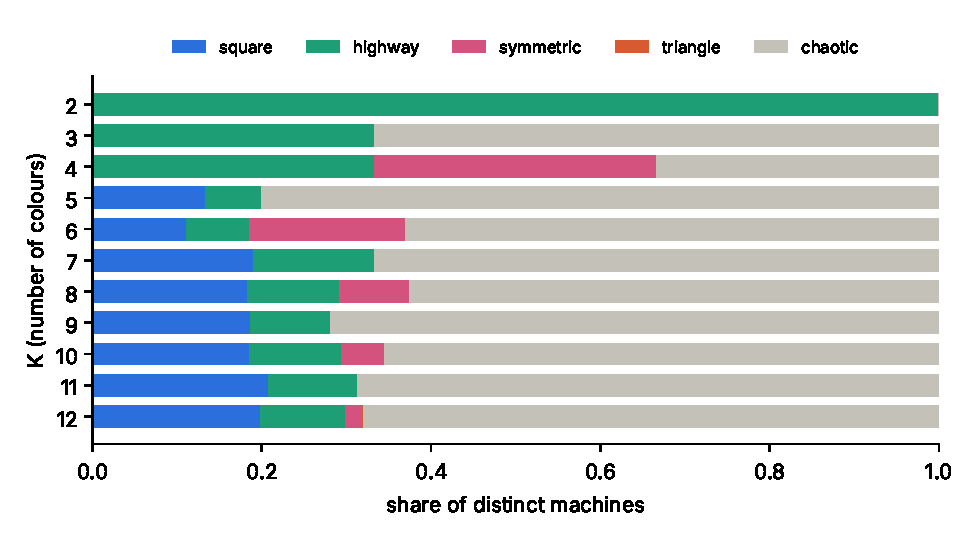
\includegraphics[width=0.85\textwidth]{../figures/shares.pdf}
\caption{Share of each class among the distinct machines with $K$ colours.}\label{fig:shares}
\end{figure}

\begin{figure}[p]
\centering
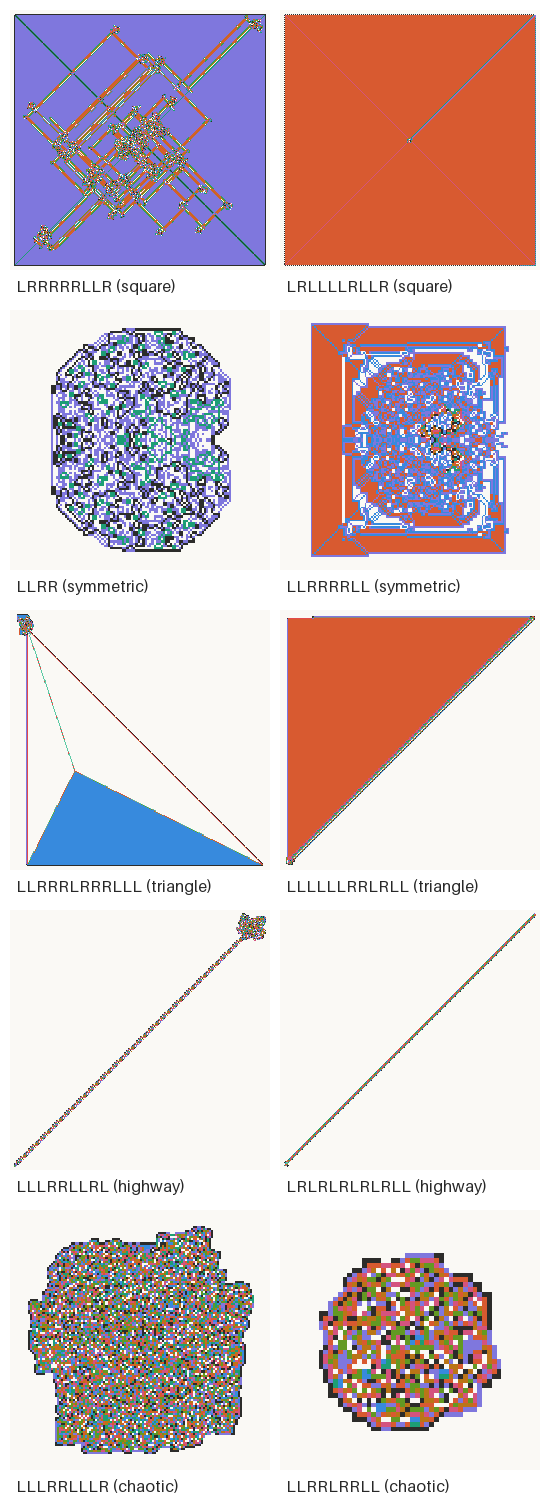
\includegraphics[height=0.86\textheight]{../figures/classes.png}
\caption{Two machines of each class, cropped to the coloured area (white is colour $0$), after $10^6$
steps; highways are shown when they reach the edge.}\label{fig:classes}
\end{figure}

About two machines in three grow a chaotic blob. From $K = 7$ on, about one in five grows a square,
roughly twice as many as build a highway. Only three triangles appear: $\Lw\Lw\Rw\Lw\Rw\Rw\Lw\Lw\Lw\Lw\Lw$
($K=11$) and $\Lw\Lw\Lw\Lw\Lw\Lw\Rw\Rw\Lw\Rw\Lw\Lw$ and $\Lw\Lw\Rw\Rw\Rw\Lw\Rw\Rw\Rw\Lw\Lw\Lw$
($K = 12$); the last is the mirror image of the known triangle rule
$\Rw\Rw\Lw\Lw\Lw\Rw\Lw\Lw\Lw\Rw\Rw\Rw$.

\section{Patterns in the rule strings}\label{sec:obs}

\begin{observation}[Even runs and symmetry]\label{obs:even}
Read a rule in a circle and split it into runs of equal letters. All $83$ symmetric machines have every
run of even length (for example $\Lw\Lw\Rw\Rw$, $\Lw\Rw\Rw\Lw$, $\Lw\Lw\Lw\Rw\Rw\Lw$).
Of the $104$ machines with this property, the other $21$ were classed square ($16$) or chaotic ($5$);
the $16$ squares are themselves highly symmetric in colour. In particular no symmetric machine exists for
odd $K$, since an odd length cannot be split into even runs.
\end{observation}

This matches the result of~\cite{gale}, which shows that such rules give patterns that are symmetric
whenever the ant returns to its starting square, not at every step; the $5$ ``chaotic'' cases are most
likely pictures taken between two such moments.

\begin{observation}[The first letters]\label{obs:prefix}
For $6 \le K \le 12$, the first three letters lean strongly towards a class:
\begin{center}
\small
\begin{tabular}{@{}lrrrr@{}}
\toprule
Rule starts with & Machines & Square & Highway & Chaotic\\
\midrule
$\Lw\Rw\Rw$ & 998 & 39\% & 0\% & 59\%\\
$\Lw\Rw\Lw$ & 997 & 18\% & 7\% & 75\%\\
$\Lw\Lw\Rw$ & 998 & 16\% & 20\% & 62\%\\
$\Lw\Lw\Lw$ & 997 & 6\% & 14\% & 76\%\\
\bottomrule
\end{tabular}
\end{center}
\end{observation}

\begin{observation}[Highways need two equal first letters, until $K = 7$]\label{obs:lr}
For $K = 3$ to $6$, every highway rule starts with $\Lw\Lw$: the ant turns the same way on a square's
first two visits. The first highway starting with $\Lw\Rw$ appears at $K = 7$
($\Lw\Rw\Lw\Lw\Rw\Rw\Lw$, which reaches the edge only at step $314{,}536$).
The numbers of highways starting $\Lw\Lw$ and $\Lw\Rw$ for $K = 3, \dots, 12$ are
$1/0$, $2/0$, $1/0$, $2/0$, $8/1$, $11/2$, $21/3$, $43/11$, $89/18$ and $163/39$.
Over all $K$, rules starting $\Lw\Lw$ build highways $17.0\%$ of the time and rules starting $\Lw\Rw$
$3.7\%$ of the time; without the copies of Section~\ref{sec:copies} the first rate is $8.8\%$.
\end{observation}

\begin{observation}[Slow growers]\label{obs:slow}
$228$ machines that are not highways are still under $40$ squares wide after $10^6$ steps.
For example $\Lw\Lw\Lw\Rw\Rw$ is $28$ squares wide after $10^6$ steps, $36$ after $1.6\times10^7$ and
$49$ after $1.024\times10^9$, gaining about four squares each time the number of steps is multiplied by
four; its picture is a slowly growing disc.
\end{observation}

\subsection{Hidden copies among the highways}\label{sec:copies}

The step at which a highway machine reaches the edge revealed that many of them are the same machine.
For instance every highway rule beginning with $\Lw\Lw\Rw\Lw\Lw\Rw$ reaches the edge at exactly step
$26{,}969$, whatever its length and later letters.

\begin{lemma}[Unread letters]\label{lem:prefix}
Suppose that, up to step $T$, the ant with rule $w$ never visits any square more than $M$ times, with
$M < |w|$. Then up to step $T$ it reads only $w_0, \dots, w_{M-1}$, and every rule that starts with
$w_0 \cdots w_{M-1}$ and has at least $M$ letters walks the same path up to step $T$.
\end{lemma}

\begin{proof}
On its $n$-th visit to a square the ant reads $w_{(n-1) \bmod |w|}$, and $n \le M < |w|$, so the
index is $n - 1 \le M - 1$. A rule $w'$ with the same first $M$ letters gives the same turn at every step,
by induction on the step.
\end{proof}

Measuring the largest number of visits to one square up to the edge, $164$ of the $416$ highway
machines never read their last letters. They fall into four families (Table~\ref{tab:copies}).
In the first three, the letters read are a shorter rule written twice, so by the repeated-strings
remark of Section~\ref{sec:defs} the path is that of the shorter ant. Grouping machines that read the
same letters, there are $252$ different highway paths among the $416$ highway machines.

\begin{table}[ht]
\centering
\caption{Highway machines that never read their last letters before reaching the edge.}\label{tab:copies}
\begin{tabular}{@{}lllrr@{}}
\toprule
Letters read & Same path as & Most visits & Reaches edge at & Copies\\
\midrule
$\Lw\Lw\Rw\Lw\Lw\Rw$ & $\Lw\Lw\Rw$ ($K=3$) & 6 & 26{,}969 & 124\\
$\Lw\Lw\Lw\Rw\Lw\Lw\Lw\Rw$ & $\Lw\Lw\Lw\Rw$ ($K=4$) & 8 & 38{,}949 & 29\\
$\Lw\Lw\Lw\Lw\Rw\Lw\Lw\Lw\Lw\Rw$ & $\Lw\Lw\Lw\Lw\Rw$ ($K=5$) & 10 & 50{,}929 & 6\\
$\Lw\Lw\Lw\Rw\Rw\Rw\Lw\Lw\Lw\Rw$ & itself ($K=10$) & 10 & 56{,}928 & 5\\
\bottomrule
\end{tabular}
\end{table}

\section{\texorpdfstring{The family $\Lw^{K-1}\Rw$}{The family L^(K-1)R}}\label{sec:family}

The first three families of Table~\ref{tab:copies} come from the rules $A_K = \Lw^{K-1}\Rw$, which turn
left on every visit to a square except each $K$-th. Their edge steps are $26{,}969$, $38{,}949$ and
$50{,}929$ for $K = 3, 4, 5$: an arithmetic progression with difference $11{,}980$.
Direct runs confirm the progression for every $K$ from $3$ to $25$ and for
$K = 30, 40, 50, 75, 100, 150, 200, 300, 500$ and $1{,}000$ (Figure~\ref{fig:formula}). In every one
of these runs the most visits to one square is exactly $2K$.

\begin{figure}[ht]
\centering
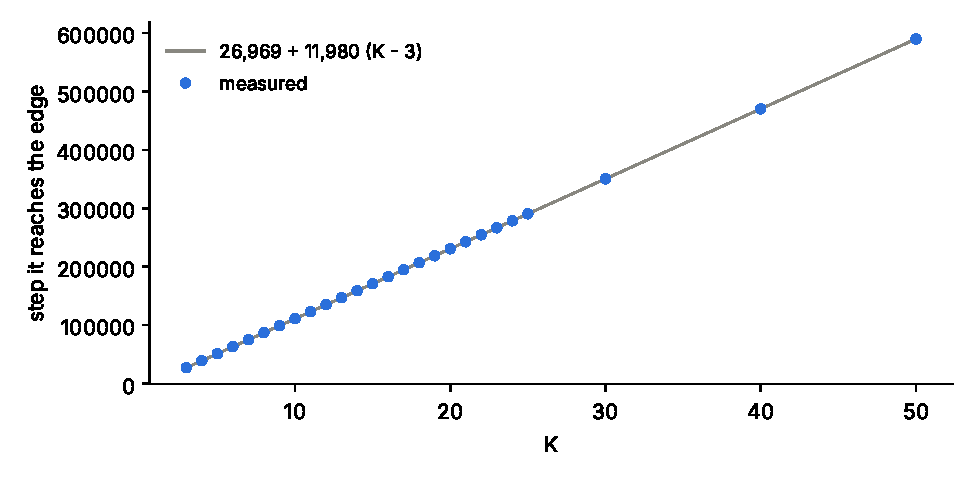
\includegraphics[width=0.85\textwidth]{../figures/lkr_formula.pdf}
\caption{Step at which $\Lw^{K-1}\Rw$ reaches the edge, measured, against $26{,}969 + 11{,}980\,(K-3)$.}
\label{fig:formula}
\end{figure}

\begin{theorem}\label{thm:main}
For every $K \ge 3$, the ant $A_K = \Lw^{K-1}\Rw$ started on an empty grid:
\begin{enumerate}[nosep,label=(\roman*)]
\item makes exactly $7{,}488$ right turns before it reaches the edge, and the $n$-th right turn happens
on the same square, leaving in the same direction, for every $K$;
\item reaches the edge at step $26{,}969 + 11{,}980\,(K - 3) = 11{,}980\,K - 8{,}971$;
\item after its $7{,}600$-th right turn, repeats forever a period of $10$ right turns that takes
$16K - 12$ steps and moves the ant by $(-2, 2)$, so it builds a diagonal highway and moves away to
infinity.
\end{enumerate}
\end{theorem}

\paragraph{Why it should be true.} Runs for $K \in \{3,4,5,6,7,10,20\}$ show the mechanism.
Between two right turns the ant makes only left turns, and four left turns in a row take it round a
$2 \times 2$ loop and back to the same square in the same direction. We call this a \emph{spin}: it adds
one visit to each of four squares per lap, until one of them reaches its letter $\Rw$. Every gap of left
turns between two consecutive right turns has the form $g_3 + \gamma\,(K-3)$ with $\gamma \in \{0,4\}$;
exactly $2{,}995$ gaps have $\gamma = 4$, and $2{,}995 \times 4 = 11{,}980$. Each extra colour adds one lap
to those spins and changes nothing else. Likewise, on every square the number of visits is the $K = 3$
number plus $m\,(K-3)$ with $m \in \{0, 1, 2\}$: whole extra cycles, which leave every square the same
number of visits away from its next $\Rw$. The proof turns these observations into a statement for all
$K$ at once.

\section{The proof}\label{sec:proof}

The proof is a computer run, \texttt{proof/symbolic.py} and \texttt{proof/highway.py} in the
repository, that follows the ant for all $K \ge 4$ simultaneously. The case $K = 3$ is a single
ordinary run (\texttt{proof/highway\_concrete.py}, Section~\ref{sec:k3}).

\subsection{Symbolic colours}

Fix $K \ge 4$. Every number the run needs is an \emph{affine expression} $a + bK$ with integers $a, b$.
We store the colour $\sigma(p) \in \{0, \dots, K-1\}$ of each square as such an expression in one of two
forms: $a + 0K$ with $a \ge 0$, or $a + 1K$ with $a \le -1$. Over the whole run the constants stay small:
$0 \le a \le 2$ in the first form and $-3 \le a \le -1$ in the second, so each expression is a genuine
colour in $\{0, \dots, K-1\}$ for every $K \ge 4$.

The run makes two kinds of decision.
\begin{enumerate}[nosep]
\item \emph{Is the ant on its $\Rw$?} For $A_K$ the ant turns right exactly when $\sigma(p) = K-1$.
The run answers \emph{yes} exactly when the stored expression is $-1 + 1K$. This is correct for every
$K \ge 4$: an expression $a + 0K$ with $a \le 2$ never equals $K - 1$, and $a + 1K$ equals $K - 1$ only if
$a = -1$.
\item \emph{Comparisons.} Whether $e = a + bK$ is positive, negative or zero for all large $K$ is decided
by the sign of $b$ (or of $a$ when $b = 0$). Each such answer holds from some $K$ on; the run records the
largest such threshold. For this run it is $K_0 = 4$.
\end{enumerate}
Equal expressions always give equal numbers, so whenever the run finds two colours equal they are equal for
every $K \ge K_0$.

\subsection{Jumping over spins}

\begin{lemma}[Spin]\label{lem:spin}
Let the ant be at square $c_0$ facing $d$, and let $c_0, c_1, c_2, c_3$ be the squares it visits if it
turns left four times (so its fourth move returns it to $c_0$ facing $d$). Let
$r_i = (K-1) - \sigma(c_i)$ be the number of visits $c_i$ can still take while reading $\Lw$, and suppose
$n = \min_i r_i \ge 1$. Then the next $4n$ steps are $n$ laps of left turns round $c_0, c_1, c_2, c_3$;
afterwards the ant is again at $c_0$ facing $d$, each $\sigma(c_i)$ has grown by $n$, and no colour has
wrapped round.
\end{lemma}

\begin{proof}
In lap $\ell \in \{1, \dots, n\}$ square $c_i$ is visited with colour
$\sigma(c_i) + \ell - 1 \le \sigma(c_i) + n - 1 \le \sigma(c_i) + r_i - 1 = K - 2$, so the ant reads
$\Lw$ there and turns left. Four left turns bring it back to $c_0$ facing $d$. After $n$ laps each
colour is $\sigma(c_i) + n \le K - 1$.
\end{proof}

The run applies Lemma~\ref{lem:spin} whenever all four $r_i$ are positive, with $n$ and the step count
$4n$ kept as affine expressions; $n$ is the least of the $r_i$, found with recorded comparisons. Otherwise
it makes one ordinary step. Positions and directions stay ordinary integers throughout, because the
order of decisions does not depend on $K$. Near the edge of $B$ spins are not jumped, so the step at which
the ant leaves $B$ is found exactly.

\subsection{Parts (i) and (ii)}

The symbolic run reaches the edge after $7{,}488$ right turns and $3{,}743$ jumped spins, with step count
$11{,}980\,K - 8{,}970$ moves, so the edge is reached at step $11{,}980\,K - 8{,}971$. Every decision on
the way holds for all $K \ge 4$. Since positions and directions in the run are integers that do not
involve $K$, the right turns are the same squares and directions for every $K \ge 4$. This proves (i) and
(ii) for $K \ge 4$.

\subsection{Part (iii): the highway goes on forever}

For the $t$-th right turn, let $p_t$ be the square where it happens, $d_t$ the direction the ant faces
after turning, $S_t$ the colouring just after that square's colour is updated, and $H_t$ the set of squares
visited so far. The ant's motion after a right turn is determined by $p_t$, $d_t$ and $S_t$.
Fix right turns $i$ and $j = i + P$, let $V$ be the set of squares visited after right turn $i$, up to and
including right turn $j$, let $D = p_j - p_i$, and let $f(c) = c \cdot D$ (dot product). Put
$A = (V + D) \setminus V$.

\begin{lemma}[Periodicity]\label{lem:period}
Suppose
\begin{enumerate}[nosep,label=(\alph*)]
\item $d_j = d_i$;
\item $S_j(c + D) = S_i(c)$ for every $c \in V$;
\item no square of $A$ is in $H_j$; and $f(D) > 0$ and $\min_{c \in A} f(c) + f(D) > \max_{c \in H_j} f(c)$.
\end{enumerate}
Then for every $k \ge 1$ the motion from right turn $i + kP$ to right turn $i + (k+1)P$ is the motion from
right turn $i$ to right turn $j$ moved by $kD$. In particular $p_{i+kP} = p_i + kD$, and the ant moves
away to infinity along $D$.
\end{lemma}

\begin{proof}
We prove by induction on $k \ge 1$ the statement
\begin{align*}
\mathcal{P}(k):\quad & p_{i+kP} = p_i + kD,\qquad d_{i+kP} = d_i,\qquad
S_{i+kP}(c + kD) = S_i(c)\ \text{for all } c \in V,\\
& H_{i+kP} = H_j \cup \textstyle\bigcup_{l=1}^{k-1}(V + lD).
\end{align*}
$\mathcal{P}(1)$ is the definition of $D$ together with (a) and (b).

Assume $\mathcal{P}(k)$. Between right turn $i$ and right turn $j$ the ant reads and writes only squares of
$V$, starting from $p_i$, $d_i$ and the colours $S_i$ on $V$. By $\mathcal{P}(k)$, at right turn $i+kP$ the
ant is at $p_i + kD$, faces $d_i$, and the colours on $V + kD$ are those of $S_i$ on $V$, moved by $kD$.
So the next $P$ right turns are the motion from $i$ to $j$ moved by $kD$: the ant visits exactly $V + kD$,
ends at $p_i + (k+1)D$ facing $d_j = d_i$, and $S_{i+(k+1)P}(c + kD) = S_j(c)$ for every $c \in V$.
This gives the position, direction and visited set in $\mathcal{P}(k+1)$. For the colours, take $c \in V$
and put $z = c + (k+1)D$.

If $c + D \in V$, then $z = (c + D) + kD$, so $S_{i+(k+1)P}(z) = S_j(c + D) = S_i(c)$ by (b).

If $c + D \notin V$, then $c + D \in A$. We claim $z$ has never been visited. First,
$f(z) = f(c + D) + k f(D) \ge \min_A f + f(D) > \max_{H_j} f$, so $z \notin H_j$. Next, if
$z \in V + lD$ with $1 \le l \le k$, then $c + (k+1-l)D \in V$. For $l = k$ this says $c + D \in V$, which
is false. For $l < k$ it says $c + mD \in V$ with $m = k + 1 - l \ge 2$; but
$f(c + mD) = f(c + D) + (m-1)f(D) \ge \min_A f + f(D) > \max_{H_j} f \ge \max_V f$, since
$V \subseteq H_j$, so this is false too. Hence $z \notin H_{i+(k+1)P}$ and $S_{i+(k+1)P}(z) = 0$.
On the other side, $S_i(c) = S_j(c + D)$ by (b), and $c + D \in A$ is not in $H_j$ by (c), so
$S_j(c+D) = 0$. Thus $S_{i+(k+1)P}(z) = S_i(c)$ in this case as well, which proves $\mathcal{P}(k+1)$.

Since $f(p_{i+kP}) = f(p_i) + k f(D)$ with $f(D) > 0$, the ant moves away to infinity.
\end{proof}

\begin{remark}
In the symbolic run, condition (b) compares affine expressions; equal expressions give equal colours for
every $K$, so (b) holds for every $K \ge 4$ at once. Conditions (a) and (c) involve only positions and
directions, which do not depend on $K$.
\end{remark}

The program \texttt{proof/highway.py} takes $i = 7{,}600$ and $P = 10$. It finds $D = (-2, 2)$, a step count
of $16K - 12$ for the period, and conditions (a), (b) (on the $18$ squares of $V$) and (c) all true, with
every decision valid for $K \ge 4$. Lemma~\ref{lem:period} gives (iii) for $K \ge 4$.

\subsection{A certificate that can be checked independently}\label{sec:cert}

So that the proof does not rest on trusting one program, the symbolic run also writes a
\emph{certificate} (\texttt{proof/certificate.txt}): a list of every action it takes up to its
$7{,}610$-th right turn, each with the numbers it depends on. There are two kinds of line: a single step
(square, direction, the square's count $a + bK$ before the visit, and the turn $\Lw$ or $\Rw$) and a spin
(square, direction, and the number of laps $n = a + bK$). The certificate has $12{,}941$ lines:
$9{,}135$ single steps, $3{,}805$ spins and one mark where the ant leaves the box $B$.

A separate program, \texttt{proof/check\_certificate.py}, which shares no code with the proof program,
replays the ant from the empty grid line by line. It makes no choices; it only checks. Every check has
the form ``$a + bK \ge c$ for every $K \ge 4$'', which holds exactly when $b \ge 0$ and $a + 4b \ge c$.
The checker verifies that:
\begin{itemize}[nosep]
\item each line's square, direction and count agree with its own replay;
\item every count stays a colour, $0 \le a + bK \le K - 1$, for every $K \ge 4$;
\item a single step turns $\Rw$ exactly when the count is $-1 + 1K = K - 1$, and turns $\Lw$ only when the
count is at most $K - 2$ for every $K \ge 4$;
\item a spin satisfies Lemma~\ref{lem:spin}: $n \ge 1$, and $n \le (K - 1) - \sigma(c_i)$ for each of its
four squares, for every $K \ge 4$; before the edge is reached, no spin touches the edge of $B$;
\item the edge mark is exactly where the replay first leaves $B$.
\end{itemize}
In total it checks $69{,}260$ inequalities, each valid for every $K \ge 4$. From its own replay it then
finds the edge after $7{,}488$ right turns at step $11{,}980K - 8{,}971$, and the three conditions of
Lemma~\ref{lem:period} at right turns $7{,}600$ and $7{,}610$, with shift $(-2,2)$ and $16K - 12$ steps per
period. As a test of the checker, we altered the certificate in several ways (one spin made one lap longer,
one left turn changed to a right turn, one line deleted); each change was rejected at the line where it was
made.


\subsection{\texorpdfstring{The case $K = 3$}{The case K = 3}}\label{sec:k3}

For $K = 3$ the rule is $\Lw\Lw\Rw$ and everything is an ordinary number. A direct run
(\texttt{src/ant\_visits.c}) reaches the edge at step $26{,}969$ after $7{,}488$ right turns
(\texttt{proof/skeleton.py} checks the right turns square by square against $K = 4, 5, 6, 7, 10, 20$),
and \texttt{proof/highway\_concrete.py} verifies conditions (a)--(c) of Lemma~\ref{lem:period} with
$i = 7{,}600$, $P = 10$, $D = (-2, 2)$ and a period of $36 = 16 \cdot 3 - 12$ steps.
This completes the proof of Theorem~\ref{thm:main}. \qed

\section{Discussion}\label{sec:discussion}

\paragraph{What the proof shows.} For $\Lw^{K-1}\Rw$ the number of colours only changes \emph{how long}
the ant spins, never \emph{where} it turns right. A single symbolic run therefore covers infinitely many
ants. The same method applies to any family of rules in which a parameter changes only the length of
spins, and could be tried on other families found in the census, for example $\Lw^{a}\Rw^{b}$ patterns.

\paragraph{Limits of the census.} The classes describe each picture after $10^6$ steps. A machine counted
as chaotic may still build a highway later: the slowest highway found took $937{,}513$ steps to reach the
edge, and for the classic ant it is not even proved that a highway must come from every finite start.
Two machines checked for $2 \times 10^9$ steps, $\Lw\Lw\Lw\Rw\Lw$ (a blob $1{,}954$ squares wide after
$1.024 \times 10^9$ steps) and $\Lw\Lw\Lw\Rw\Rw$ (a disc $49$ squares wide), built no highway in that
time. The tests are rough: a few blobs sit inside square frames, and one wedge-shaped machine,
$\Lw\Lw\Rw\Lw\Rw\Rw\Lw\Lw\Lw$, grows a chequered arrowhead that has no class of its own and is counted as
chaotic. All runs start from an empty grid.

\paragraph{Further work.} Natural next steps are (1) running the chaotic machines much longer to find late
highways; (2) a census with the copies of Section~\ref{sec:copies} removed for every class, not only
highways; (3) proving the even-runs pattern and the slow ``disc'' growth; and (4) submitting the count
sequences by $K$ to the OEIS once they are stable.

\section*{Code and data availability}

All code and data, including the proof certificate and its checker, are in the repository
\begin{center}\url{https://github.com/VishnuVaidyanathan/langtons-ant-census}\end{center}
The script \texttt{run\_all.sh} rebuilds every
number, table and figure in this paper in about two minutes on a laptop. Appendix~\ref{app:code} lists
the files.

\section*{Acknowledgements}

The author thanks Claude (Anthropic) for help with programming, running the computations, and drafting.

\begin{thebibliography}{9}

\bibitem{langton}
C.~G. Langton.
\newblock Studying artificial life with cellular automata.
\newblock \emph{Physica D}, 22:120--149, 1986.

\bibitem{dewdney}
A.~K. Dewdney.
\newblock Computer recreations.
\newblock \emph{Scientific American}, 261(3), September 1989.

\bibitem{gale}
D.~Gale, J.~Propp, S.~Sutherland and S.~Troubetzkoy.
\newblock Further travels with my ant.
\newblock \emph{The Mathematical Intelligencer}, 17(3):48--56, 1995.

\bibitem{bunimovich}
L.~A. Bunimovich and S.~E. Troubetzkoy.
\newblock Recurrence properties of Lorentz lattice gas cellular automata.
\newblock \emph{Journal of Statistical Physics}, 67:289--302, 1992.

\bibitem{gajardo}
A.~Gajardo, A.~Moreira and E.~Goles.
\newblock Complexity of Langton's ant.
\newblock \emph{Discrete Applied Mathematics}, 117:41--50, 2002.

\end{thebibliography}

\appendix
\section{Repository contents}\label{app:code}

\begin{center}
\small
\begin{tabular}{@{}lp{8.6cm}@{}}
\toprule
File & Purpose\\
\midrule
\texttt{run\_all.sh} & Rebuilds everything from scratch.\\
\texttt{src/ant\_census.c} & Runs all $2^K$ rule strings for one $K$; prints shape measures.\\
\texttt{src/classify.py} & Removes repeated strings and mirror twins; assigns classes.\\
\texttt{src/analyse.py} & All numbers of Sections~\ref{sec:census}--\ref{sec:family}.\\
\texttt{src/ant\_visits.c} & Edge step and most visits to one square for one rule.\\
\texttt{src/ant\_snap.c}, \texttt{src/make\_figures.py} & Figures.\\
\texttt{proof/symbolic.py} & Symbolic run: Theorem~\ref{thm:main}(i)--(ii) for $K \ge 4$.\\
\texttt{proof/highway.py} & Symbolic periodicity check: Theorem~\ref{thm:main}(iii) for $K \ge 4$.\\
\texttt{proof/write\_certificate.py} & Writes the certificate \texttt{proof/certificate.txt}.\\
\texttt{proof/check\_certificate.py} & Independent checker of the certificate (Section~\ref{sec:cert}).\\
\texttt{proof/highway\_concrete.py} & The same check with plain numbers, used for $K = 3$.\\
\texttt{proof/skeleton.py} & The observations behind the proof, for several $K$.\\
\texttt{data/census.csv} & The $4{,}015$ distinct machines with class and measures.\\
\texttt{data/census\_raw.csv} & Measures for all $8{,}188$ rule strings.\\
\texttt{data/highways.txt}, \texttt{data/squares.txt} & Highway and square machines by $K$.\\
\bottomrule
\end{tabular}
\end{center}

\end{document}
